\chapter{Computational details}
This chapter provides detailed information on the computational methods employed in this work. The first section outlines the generation of the training dataset, including system preparation, initial equilibration using molecular mechanics, exploration of the configuration space at the GFN1-xTB level, further data labelling, and iterative training of the neural network potential. The second section discusses production runs at ambient temperature using the fitted neural network potential. Finally, the third section presents the data analysis and visualisation techniques used to interpret the results.



%%%%%%%%%%%%%%%%%%%%%%%%%%%%%%%%%%%%%%%%%%%%%%%%%%%%%%%%%%%%%%%%%%%%%%%%%%%%%%%%

\section{Training dataset generation}

\subsection{System preparation}
The systems were prepared using the functionality of the CHARMM-GUI webserver \citep{joCHARMMGUIWebbasedGraphical2008}, specifically the Multicomponent Assembler interface~\citep{kernCHARMMGUIMulticomponentAssembler2024}.

As a first step, \acf{medp} and \acf{mehdp} were parameterised using CGenFF~\citep{kimCHARMMGUILigandReader2017}, i.e., the CHARMM General Force Field. These protonation states were chosen based on the dissociation constants of pyrophosphoric (diphosphoric) acid~\citep{haynesCRCHandbookChemistry2016}:
\begin{align*}
    \mathrm{H_4P_2O_7} \rightleftharpoons \mathrm{[H_3P_2O_7]^-} + \mathrm{H^+},\quad \mathrm{p}K_\mathrm{a} = 0.91 \\
    \mathrm{[H_3P_2O_7]^-} \rightleftharpoons \mathrm{[H_2P_2O_7]^{2-}} + \mathrm{H^+},\quad \mathrm{p}K_\mathrm{a} = 2.10 \\
    \mathrm{[H_2P_2O_7]^{2-}} \rightleftharpoons \mathrm{[HP_2O_7]^{3-}} + \mathrm{H^+},\quad \mathrm{p}K_\mathrm{a} = 6.70 \\
    \mathrm{[HP_2O_7]^{3-}} \rightleftharpoons \mathrm{[P_2O_7]^{4-}} + \mathrm{H^+},\quad \mathrm{p}K_\mathrm{a} = 9.32
\end{align*}

Thus, at physiological pH (7.4), this acid exists in equilibrium between the singly and doubly deprotonated forms. Assuming the methyl group behaves similarly to a proton, the methyl diphosphate molecule was considered to exist as a mixture of the \ac{mehdp} and \ac{medp} forms under physiological conditions.

Following successful parameterisation, the system was solvated in a cubic box of TIP3P water molecules, with sodium counterions (Na\textsuperscript{+}) added to neutralise the system's overall charge. The final system composition is provided in Table~\ref{tab:system-before-equilibration}.



\subsection{Initial equilibration using classical force fields}
The system equilibration followed the standard protocol generated by the CHARMM-GUI webserver~\citep{joCHARMMGUIWebbasedGraphical2008}. Initially, energy minimisation was conducted using the steepest descent algorithm for 5,000 steps.

This was followed by equilibration in the \ac{nvt} ensemble for 5 ns. During both the minimisation and \ac{nvt} phases, the solute's heavy atoms were restrained using a harmonic potential with a force constant of 400 kJ mol\textsuperscript{-1} nm\textsuperscript{-2}.

Subsequently, the system was equilibrated in the \ac{npt} ensemble for 45 ns. Throughout this procedure, the temperature and pressure were maintained at 300 K and 1 bar, respectively. Temperature was controlled using a $\nu$-rescale thermostat~\citep{bussiCanonicalSamplingVelocity2007} with a coupling constant of 1 ps, and pressure was regulated using an isotropic \textit{c}-rescale barostat~\citep{bernettiPressureControlUsing2020} with a coupling constant of 5 ps. A 0.6 nm cut-off was applied for non-bonded interactions, and long-range electrostatics were treated using the \ac{pme} method. \Ac{pbc} were applied in all directions throughout the simulation.

\begin{table}[b]
    \centering
    \caption{System composition and simulation box details.}
    \label{tab:system-before-equilibration}
    \begin{tabular}{ccccc}
    \toprule
    \textbf{System} & \textbf{Final box dimensions (\AA\textsuperscript{3})} & \textbf{No. of H\textsubscript{2}O} & \textbf{No. of Na\textsuperscript{+}} & \textbf{No. of atoms} \\
    \midrule
    MeDP  & $15.877 \times 15.877 \times 15.877$ & 119 & 3 & 373 \\
    MeHDP & $15.901 \times 15.901 \times 15.901$ & 124 & 2 & 388 \\
    \bottomrule
    \end{tabular}
\end{table}

All simulations were carried out using GROMACS 2021.4~\citep{abrahamGROMACSHighPerformance2015} with CHARMM36m force field~\citep{huangCHARMM36mImprovedForce2017}. The leap-frog integrator was employed with a time step of 1 fs. All hydrogen-involving bonds were constrained using the LINCS algorithm. The equilibrated box dimensions used for subsequent simulations were taken from the output of the \ac{npt} run and are summarised in Table~\ref{tab:system-before-equilibration}. Unless otherwise stated, the last frame of the \ac{npt} simulations was used as the starting point for all further calculations.



\subsection{Collective variables}
To effectively sample the reaction space, two types of \acp{cv} were employed to bias the system: distances and \acp{cn}. The \ac{cn} is defined by the following smooth function:
\begin{equation}
    \sum_{i \in A} \sum_{j \in B} CN_{ij} = \frac{1 - \left( \frac{r_{ij} - d_0}{r_0} \right)^n}{1 - \left( \frac{r_{ij} - d_0}{r_0} \right)^m}
    \label{eq:coordination_number}
\end{equation}
where $r_{ij}$ is the distance between atoms $i$ and $j$ from groups $A$ and $B$, $d_0$ is the distance at which the \ac{cn} begins to decay, $r_0$ is a characteristic decay length, and $n$ and $m$ are integers that control the steepness of the decay. Typically, $m > n$, ensuring a smooth transition of $CN_{ij}$ from approximately 1 to 0 as the distance increases.

The specific \acp{cv} used in this work are shown in Figure~\ref{fig:collective_variables}, and their corresponding parameters are as follows:

\begin{itemize}
    \item Distance between the $\beta$-phosphorus and the bridging oxygen (d\textsubscript{P-O\textsubscript{lg}}),
    \item Coordination number of all water oxygen atoms as well as the bridging oxygen surrounding the $\beta$-phosphorus (C\textsubscript{P-O\textsubscript{all}}): $d_0 = 0$, $r_0 = 2.1$ \AA, $n = 8$, $m = 16$.
\end{itemize}

\begin{figure}[b!]
    \centering
    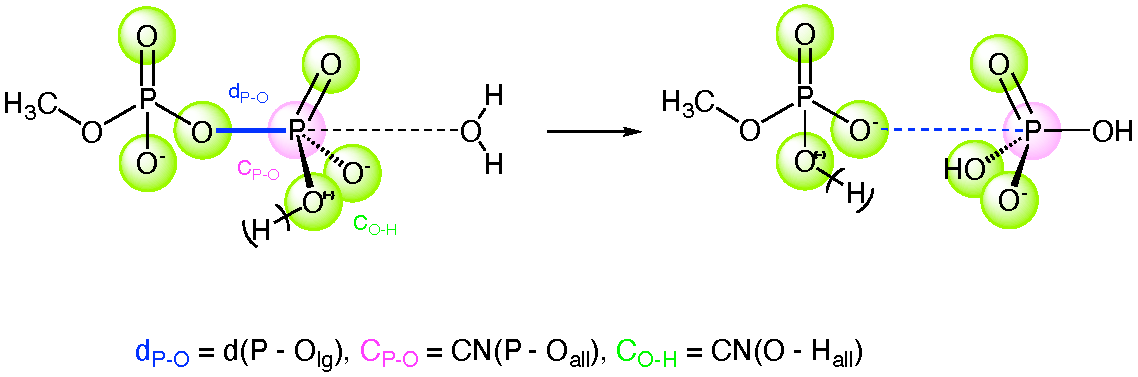
\includegraphics[width=0.95\textwidth]{Figures/3_Computational_details/methods_collective_variables.pdf}
    \caption{The definition of the collective variables (CVs) used in this work. d stands for distance and CN stands for coordination number.}
    \label{fig:collective_variables}
\end{figure}

Additionally, the following \acp{cv} were monitored to check whether the system was in a reasonable region of the potential energy surface, e.g. to ensure that there is no oxygen exchange between the methyl diphosphate and the water molecules:
\begin{itemize}
    \item Coordination number of 3 nonbridging phosphoryl oxygens surrounding the $\beta$-phosphorus (C\textsubscript{P-O\textsubscript{nb}}): $d_0 = 0$, $r_0 = 2.1$ \AA, $n = 8$, $m = 16$,
    \item Coordination number of 2 nonbridging oxygens from $\alpha$-phosphorus as well as the one forming a bond with the methyl group surrounding the $\beta$-phosphorus (C\textsubscript{P-O\textsubscript{nb-lg}}): $d_0 = 0$, $r_0 = 2.1$ \AA, $n = 8$, $m = 16$,
    \item Coordination number of water oxygens around the $\beta$-phosphorus (C\textsubscript{P-O\textsubscript{w}}): $d_0 = 0$, $r_0 = 2.1$ \AA, $n = 8$, $m = 16$,
    \item Coordination number of non-methyl hydrogen atoms around 5 non-bridging and 1 bridging oxygen atoms (C\textsubscript{O-H\textsubscript{all}}): $d_0 = 0$, $r_0 = 1.3$ \AA, $n = 8$, $m = 16$.
\end{itemize}

To avoid sampling of unphysical regions of the potential energy surface, quadratic (harmonic-like) wall potentials were applied to softly constrain certain degrees of freedom. The mathematical form of these wall potentials is given below:
\begin{equation}
    \text{For upper walls:} \; \sum_i k_i \left( \frac{CV_i - a_i + o_i}{s_i} \right)^{e_i}
    \label{eq:upper_wall}
\end{equation}
\begin{equation}
    \text{For lower walls:} \; \sum_i k_i \left| \frac{CV_i - a_i - o_i}{s_i} \right|^{e_i}
    \label{eq:lower_wall}
\end{equation}
Here, $CV_i$ denotes the value of the collective variable, $k_i$ is the force constant defining the wall's strength, $a_i$ is the central wall position, $o_i$ is an offset, $s_i$ is a scaling factor, and $e_i$ is the exponent that controls the wall's steepness. When $e_i = 2$, the potential acts harmonically.

The wall potentials applied to the \acp{cv} during the simulations are summarised in Table~\ref{tab:wall_potentials}. The parameters for the wall potentials were chosen based on the expected ranges of the \acp{cv}. The force constants were set to ensure that the walls were sufficiently strong to prevent unphysical configurations while allowing for reasonable exploration of the configuration space.

\begin{table}[b!]
    \centering
    \caption{The restraints applied to the collective variables during some of the simulations. In all cases, $o = 0$, $s = 1$, $e = 2$. \textsuperscript{1}During the iterative training / production runs. \textsuperscript{2}Different values for the walls were used depending on the system MeDP/MeHDP. Distances are in \AA\ and coordination numbers are unitless.}
    \label{tab:wall_potentials}
    \begin{tabular}{cccc}
    \toprule
    \textbf{CV} & \textbf{Lower wall} & \textbf{Upper wall} & \textbf{Force constant (kcal mol\textsuperscript{-1} \AA\textsuperscript{-2})} \\
    \midrule
    d\textsubscript{P-O\textsubscript{lg}} & -- & 5.0 / 6.0$^{1}$ & 500  \\
    C\textsubscript{O-H\textsubscript{all}} & -- & 1.3 / 2.5$^{2}$ & 1000 \\
    C\textsubscript{P-O\textsubscript{nb}} & 2.6 & -- & 2000 \\
    C\textsubscript{P-O\textsubscript{nb-lg}} & -- & -- / 0.1$^{1}$ & 2000 \\
    C\textsubscript{P-O\textsubscript{w}} & -- & 1.3 & 2000 \\
    \bottomrule
    \end{tabular}
\end{table}

All \ac{cv}-related computations were performed using the built-in tools of CP2K 2023.1 \citep{kuhneCP2KElectronicStructure2020} or PLUMED 2.9.3~\citep{tribelloPLUMED2New2014}. It is important to note that the number and type of \acp{cv}, as well as the applied restraints, varied depending on the specific stage of the workflow. In the following sections, the relevant collective variables and wall potentials will be specified accordingly.



\subsection{GFN1-xTB based exploration of the configuration space}
\label{subsec:xtb-exploration-of-configuration-space}
To generate the initial set of configurations for the training dataset, the system was subjected to molecular dynamics simulations using the semi-empirical GFN1-xTB~\citep{grimmeRobustAccurateTightBinding2017} level of theory. 

Each system was first equilibrated for 5 ps in the \ac{nvt} ensemble at 300 K to allow the structures to relax at the GFN1-xTB level, including a Grimme's D3 dispersion correction~\citep{grimmeConsistentAccurateInitio2010}. Following equilibration, we performed 50 ps of \ac{wtmd}~\citep{barducciWellTemperedMetadynamicsSmoothly2008} simulations in the \ac{nvt} ensemble. In these simulations, a biasing potential was applied to encourage the system to explore regions of the configuration space beyond the reactant basin. This bias was introduced along two \acp{cv}: the distance between the $\beta$-phosphorus and the oxygen atom connecting it to the rest of the molecule (d\textsubscript{P-O}), and the coordination number of all water oxygens together with the bridging oxygen surrounding the $\beta$-phosphorus atom (C\textsubscript{P-O}). No restraints were applied to the system during this stage.

All calculations were carried out using the CP2K 2023.1 package~\citep{kuhneCP2KElectronicStructure2020} on CPUs. Temperature control was achieved using the \ac{csvr} thermostat~\citep{bussiCanonicalSamplingVelocity2007}, with a time constant of 50 fs during equilibration and 100 fs during the \ac{wtmd} simulations. The \ac{scf} convergence threshold was set to $10^{-5}$ a.u. The biasing potential was updated every 25 fs, with a Gaussian hill height of 2 kcal mol\textsuperscript{-1} and a width of 0.07 for each \ac{cv}. The bias factor was set to 30. Finally, the integration time step was set to 0.5 fs. Throughout the simulations, \ac{pbc} were applied in all directions.



\subsection{Data labeling}
All data points were labeled by performing single-point calculations to obtain the energy and force values. These single-point calculations were carried out using the \ac{pbe}~\citep{perdewGeneralizedGradientApproximation1996}, along with a Grimme's D3 dispersion correction and the Becke-Johnson damping function~\citep{grimmeConsistentAccurateInitio2010,grimmeEffectDampingFunction2011}. In all calculations, the \ac{gth}~\citep{goedeckerSeparableDualspaceGaussian1996,hartwigsenRelativisticSeparableDualspace1998} were used to represent the core electrons, in combination with the \ac{tzv2p}.

The single-point calculations were performed using the \; \ac{gpw} implemented in the QUICKSTEP module~\citep{vandevondeleQuickstepFastAccurate2005} of the CP2K 2023.1 package~\citep{kuhneCP2KElectronicStructure2020}. The \ac{scf} convergence threshold was set to 10\textsuperscript{-6} a.u. A plane-wave cutoff of 800 Ry was applied for the total density, while a cutoff of 60 Ry was used for the Kohn-Sham orbitals.

The aforementioned cutoffs were determined based on a convergence test performed on one of the configurations, as described in~\citep{cp2k_developersHowConvergeCUTOFF}. An error in total energy of less than 10\textsuperscript{-8} a.u. was considered acceptable for the convergence test. The test was conducted by varying the cutoff for the total density from 400 to 1500 Ry, and the cutoff for the Kohn-Sham orbitals from 10 to 200 Ry. The results of the convergence test are shown in Table~\ref{tab:cutoff-convergence-test}.

After the \ac{dft} labelling, the data were transformed into the extended XYZ format, which includes atomic positions, forces, total energies, cell dimensions, and whether \ac{pbc} were used or not. This format was chosen because it is compatible with neural network training, as explained in the next section. The data transformation was carried out using an in-house script, \texttt{cp2k2extxyz.py}, which is available in~\citep{makhmudovCp2k_to_extxyzScriptThat}.



\subsection{Iterative training of the neural network potential} \label{subsec:iterative-training-of-the-neural-network-potential}
We trained a \ac{nnp} using the NequIP framework~\citep{batznerE3equivariantGraphNeural2022}, which implements equivariant message-passing networks for atomistic simulations. Regarding the hyperparameters, a radial cutoff distance of 5.0 \AA\ was chosen to describe the atomic environment of the system.

The equivariant part of the neural network was composed of four interaction layers with a maximum tensor rank of $\ell = 1 \; \text{or} \; 2$. Feature parity was enabled to include both even and odd components, and 32 features per irreducible representation were used throughout. Scalar and gating nonlinearities were set to \texttt{silu} and \texttt{tanh} for even and odd parities, respectively. Eight radial basis functions were employed, in combination with a trainable Bessel basis and a polynomial cutoff of order 6.

The invariant subnetwork for radial interaction modelling consisted of two layers with 64 hidden neurons. Self-connections were enabled, and the average number of neighbours was computed automatically based on the dataset.

\begin{figure}[t!]
    \centering
    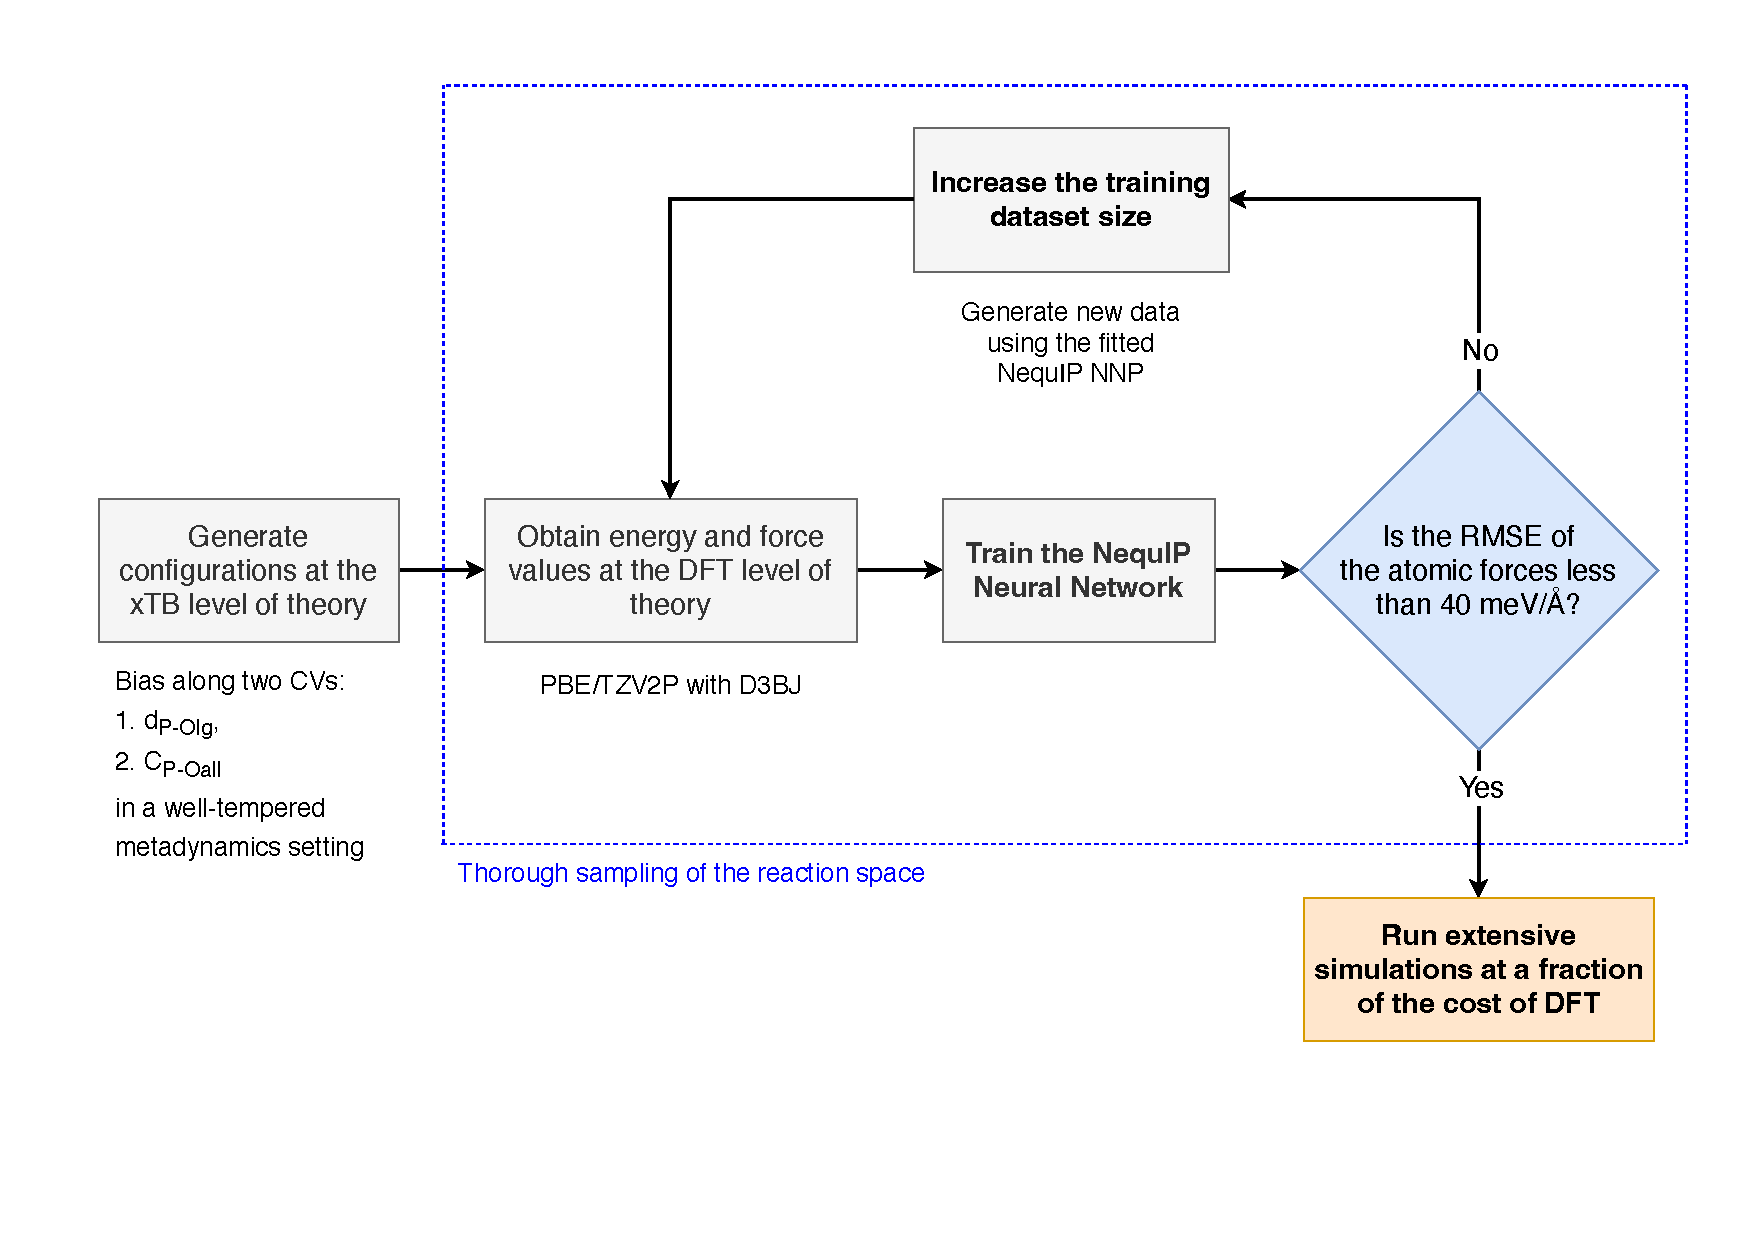
\includegraphics[width=0.95\textwidth]{Figures/3_Computational_details/methods_workflow_diagram.pdf}
    \caption{Iterative training of the NequIP neural network potential.}
    \label{fig:iterative-training}
\end{figure}

Training was performed using the Adam optimizer with the AMSGrad variant enabled, and with $\beta_1 = 0.9$, $\beta_2 = 0.999$, and $\epsilon = 10^{-8}$. A starting learning rate of 0.01 was used, and the learning rate was adaptively reduced by a factor of 0.5 upon stagnation of the validation loss (patience = 100 epochs). Early stopping was triggered if the validation loss remained unimproved for 50 epochs, if the loss dropped below $1 \times 10^{-5}$, or if it exceeded $1 \times 10^{4}$. The batch size was set to 5. The training was carried out over a period of three days on a single NVIDIA A100 GPU using float64 precision.

The networks were trained using the following \ac{mse} loss function already implemented in the NequIP framework:

\begin{equation}
    \mathcal{L} = \lambda_E \lVert \hat{E} - E \rVert^2 
    + \lambda_F \frac{1}{3N} \sum_{i=1}^{N} \sum_{\alpha=1}^{3} 
    \left\lVert -\frac{\partial \hat{E}}{\partial r_{i,\alpha}} - F_{i,\alpha} \right\rVert^2
    \label{eq:loss_function}
\end{equation}

Here, $N$ is the number of atoms, $\hat{E}$ is the predicted energy, $E$ is the reference energy, $F_{i,\alpha}$ is the reference force on atom $i$ in direction $\alpha$, and $-\frac{\partial \hat{E}}{\partial r_{i,\alpha}}$ is the calculated force by means of autodifferentiating the predicted energy with respect to the atomic position. The hyperparameters $\lambda_E$ and $\lambda_F$ by default have a weighting of 1 to $N_{atoms}^2$, respectively.

To thoroughly sample the reaction space, the training was performed in an iterative manner, where the model was first trained on a small set of data and then used to generate additional data points. This process was repeated until the model converged, with the \ac{rmse} of the atomic forces being less than 40 meV/\AA. The workflow is shown in Figure~\ref{fig:iterative-training}.

In the end, the full dataset consisted of 12,000 configurations for training and validation, and 1,800 configurations for testing, for both systems (\ac{medp} and \ac{mehdp}) combined. This dataset was obtained within the three rounds of iterative training. In each round of training, the model was retrained on a larger dataset. The data obtained from each round will be discussed in the following sections.



\subsubsection{Selection of configurations for training and testing}

An important part of the iterative training process is the selection of configurations that will be used to train the neural network. To construct a representative and diverse dataset for training the neural network potential, configurations were selected from a metadynamics trajectory using a density-aware sampling strategy. The raw data were extracted from a file generated during the enhanced sampling simulations. Each configuration in this file corresponds to a simulation snapshot, annotated with a time index and two collective variables (CVs): the distance d\textsubscript{P-O\textsubscript{lg}} and the coordination number C\textsubscript{P-O\textsubscript{all}}.

The two \acp{cv} were combined into a two-dimensional feature space $\mathbf{X} = (\mathrm{d}, \mathrm{C})$, which served as the basis for sampling. This feature space often exhibits regions of highly non-uniform data density, due to the biased nature of metadynamics sampling. To account for this, a density-aware sampling method was employed to select configurations for training and testing that maintain good coverage across the feature space.

The selection procedure proceeds as follows:
\begin{enumerate}
    \item A user-defined number of samples is specified.
    \item K-means clustering is applied to the feature space to partition it into a number of clusters, $k$. The number of clusters is determined heuristically as $k = \max\left(10, \; \min\left(\left\lfloor \frac{N}{50} \right\rfloor, \left\lfloor \frac{n_\text{samples}}{10} \right\rfloor \right)\right)$, where $N$ is the total number of configurations and $n_\text{samples}$ is the desired number of samples.
    \item The number of points sampled from each cluster is proportional to its size, ensuring that denser regions do not dominate the dataset. A minimum of one sample is taken from each non-empty cluster.
    \item Within each cluster, a fixed number of configurations is randomly selected using a deterministic random seed to ensure reproducibility.
    \item After the training set is selected, the remaining configurations are used to construct the test set, following the same density-aware procedure while ensuring no overlap with the training configurations.
\end{enumerate}

This approach results in training and test datasets that closely mirror the overall distribution of the \acp{cv}, while ensuring that underrepresented regions of the feature space are adequately sampled. The final output consists of two lists of snapshot indices corresponding to the selected training and test configurations, along with their respective \ac{cv} values. These snapshots were then extracted from the trajectory files for use in model training and evaluation. The pseudo-code for the density-aware sampling algorithm is provided in Algorithm~\ref{alg:density_aware_sampling}.



\subsubsection{First round}
In the first round of training the \ac{nnp}, the model was trained on a small dataset consisting of 4,000 configurations. These configurations were obtained from the initial exploration of the configuration space at 300~K using the GFN1-xTB level of theory, as described in Section~\ref{subsec:xtb-exploration-of-configuration-space}. The enhanced sampling simulations were biased along d\textsubscript{P-O\textsubscript{lg}} and C\textsubscript{P-O\textsubscript{all}}, and no restraints were applied to the system. The training was carried out using the hyperparameters described in Section~\ref{subsec:iterative-training-of-the-neural-network-potential}.



\subsubsection{Second round}
In the second round of training, the model was trained on a larger dataset consisting of 8,000 configurations. The additional configurations were obtained from a second round of exploration of the configuration space, driven by the \ac{nnp} obtained after the first round of training.

The \ac{nnp}-driven simulations were run using the LAMMPS package~\citep{thompsonLAMMPSFlexibleSimulation2022} compiled with PLUMED 2.9.3~\citep{tribelloPLUMED2New2014} and \texttt{pair\_nequip}~\citep{MirgroupPair_nequip} on a single A100 GPU. The simulations were performed for 100~ps in the \ac{nvt} ensemble at 300~K with the \ac{pbc} applied in all directions. The temperature was controlled by a Nos\'e--Hoover thermostat~\citep{noseUnifiedFormulationConstant1984, hooverCanonicalDynamicsEquilibrium1985} with a time constant of 50~fs. The biasing potential was applied to d\textsubscript{P-O\textsubscript{lg}} and C\textsubscript{P-O\textsubscript{all}} every 50~fs, using a Gaussian hill height of 2~kcal~mol\textsuperscript{-1} and a width of 0.07 for each CV. The bias factor was set to 30, and the integration time step was 0.5~fs.

Restraints were applied to d\textsubscript{P-O\textsubscript{lg}} and C\textsubscript{P-O\textsubscript{all}} in order to favour either a dissociative or associative mechanism of the reaction and sample more configurations from the \ac{ts} regions. The training was performed using the same hyperparameters as in the first round.



\subsubsection{Third round}
In the final round of training, the model was trained on a dataset consisting of 12,000 configurations. These additional configurations were obtained from a third round of exploration of the configuration space, driven by the \ac{nnp} obtained after the second round of training. The simulations were performed for 500~ps using the same setup as in the second round. The only difference was that the temperature in this round was increased to 320~K and 340~K to explore the configuration space at higher temperatures. The same \acp{cv} were biased as in the previous run. No restraints were applied to the system. The training was conducted using the same hyperparameters as in the first round. The final dataset is summarised in Table~\ref{tab:full_dataset}.



%%%%%%%%%%%%%%%%%%%%%%%%%%%%%%%%%%%%%%%%%%%%%%%%%%%%%%%%%%%%%%%%%%%%%%%%%%%%%%%%

\section{Production runs at ambient temperature}
To thoroughly sample the reaction space, the long production runs were performed at ambient temperature (300~K) using the neural network potential obtained in the final round of training. To run the simulations with the \ac{nnp}, the LAMMPS package~\citep{thompsonLAMMPSFlexibleSimulation2022}, compiled with PLUMED 2.9.3~\citep{tribelloPLUMED2New2014} and \texttt{pair\_nequip}~\citep{MirgroupPair_nequip}, was utilised. First, the systems were equilibrated for 75 ps in \ac{nvt} ensemble, since it was previously shown that water fully relaxes in this timeframe~\citep{moronMacroNanoScale2016}. Then the simulations were carried out for 2~ns in the \ac{nvt} ensemble, with temperature regulated by a Nos\'e--Hoover thermostat~\citep{noseUnifiedFormulationConstant1984, hooverCanonicalDynamicsEquilibrium1985} with a frequency of 50~fs\textsuperscript{-1}.

The biasing potential was applied every 50~fs to d\textsubscript{P-O\textsubscript{lg}} and C\textsubscript{P-O\textsubscript{all}} using a Gaussian hill height of 0.5~kcal~mol\textsuperscript{-1} and a width of 0.07 for each collective variable. Additionally, restraints were imposed on the \acp{cv} as mentioned in Table~\ref{tab:wall_potentials}. The bias factor was set to 30, and the integration time step was maintained at 0.5~fs. All simulations were conducted on a single A100 GPU.

To obtain the free energy profiles of the reactions, the Gaussian kernels applied during the simulations were summed using the \texttt{sum\_hills} utility provided in the PLUMED 2.9.3 package~\citep{tribelloPLUMED2New2014}. Afterwards, the \acp{mfep} were extracted using the MEPSA 1.4 software~\citep{marcos-alcaldeMEPSAMinimumEnergy2015}. 

% Having \acp{mfep} in hand and the barrier heights as a consequence, the corresponding rate constants (in s\textsuperscript{-1}) were calculated using the Eyring-Polanyi equation:
% \begin{equation}
%     k = \frac{\kappa k_B T}{h} e^{-\Delta G^\ddagger / RT}
% \end{equation}
% where the transmission coefficient $\kappa = 1$. Subsequently, the Arrhenius relationship was derived to obtain the activation energy barrier as the slope of the linear fit from the \(\log(k)\) versus \(1000/T\) plot.

% With the rate constants determined, the corresponding half-lives were then calculated using the following equation:
% \begin{equation}
%     t_{1/2} = \frac{\ln(2)}{k}
%     \label{eq:half_life}
% \end{equation}



%%%%%%%%%%%%%%%%%%%%%%%%%%%%%%%%%%%%%%%%%%%%%%%%%%%%%%%%%%%%%%%%%%%%%%%%%%%%%%%%

% \section{Validation of the transition states}



%%%%%%%%%%%%%%%%%%%%%%%%%%%%%%%%%%%%%%%%%%%%%%%%%%%%%%%%%%%%%%%%%%%%%%%%%%%%%%%%

% \section{Lifetime of the transition states}



%%%%%%%%%%%%%%%%%%%%%%%%%%%%%%%%%%%%%%%%%%%%%%%%%%%%%%%%%%%%%%%%%%%%%%%%%%%%%%%%

\section{Data analysis and visualisation}
Data analysis was performed using Python in Jupyter notebooks~\citep{grangerJupyterThinkingStorytelling2021}. All plots were generated using Matplotlib library~\citep{hunterMatplotlib2DGraphics2007}. The water oxygen-oxygen $g_\mathrm{O-O}(r)$ \ac{rdf} was calculated using the extension in VMD~\citep{humphreyVMDVisualMolecular1996} with the bin size of 0.0125~\AA\ using the 2 ns of the production runs.
